\documentclass{article}
\title{ECE 478-- Homework 7}
\usepackage{graphicx}
\usepackage{fancyhdr}
\usepackage{enumitem}
\usepackage{amsmath}
\usepackage{amssymb}
\usepackage{float}
\usepackage{amsmath}
\usepackage[margin=1in]{geometry}
\pagestyle{fancy}
\fancyhf{}
\fancyhead[L]{Gianni Avilan-Losee}
\fancyhead[C]{ECE 478}
\fancyhead[R]{Homework 8}
\fancyfoot[C]{\thepage}
\usepackage{microtype}
\usepackage{textcomp, gensymb}
\author{Gianni Avilan-Losee}
\begin{document}
\setcounter{section}{10}
\setcounter{subsection}{23}
\begin{enumerate}[label=\thesubsection]
	\item Using the formula for mean time between failures (MTBF),
		\[
			\mathrm{MTBF} = \frac{T_ce^{\frac{T_c}{\tau_s}}}{NT_0},
		\]
		we may calculate the minimum clock period for an MTBF of 100 years \((100\pi \times 10^7)\) as 
		\[
			100\pi \times 10^7 = \frac{T_ce^{\frac{T_c}{54 \times 10^{-12}}}}{10^7 \times 21 \times 10^{-12}} \Leftrightarrow T_c \approx 1.81 \times 10^{-9} \ \mathrm{s},
		\]
		or a maximum clock frequency of 
		\[
			\frac{1}{T_c} = 0.553 \times 10^9 =  553 \ \mathrm{MHz}.
		\]
		\setcounter{section}{11}
		\setcounter{subsection}{2}
	\item In two's complement addition, overflow will never occur due to the sum of a positive and negative number, so we only need to worry about conditions where we are summing to positive numbers or two negative numbers. Overflow occurs when the sum of two negative numbers is positive, or the sum of two positive numbers is negative. Since the MSB of each two's complement number is its sign bit, the two conditions that correspond to overflow are \(110\) and \(001\), if the sign bits of the two summands are represented by the two most significant bits, and the sign bit of the sum is the least significant bit. Representing these three values as \(A,B,\) and \(C\), respectively, we may develop a Boolean expression that outputs 1 for overflow as
		\[
			(AB\overline{C}) + \overline{(AB\overline{C})}.
		\]
		\setcounter{subsection}{6}
	\item Extrapolating from the design of the adder and the available bits for summation as a function of the number of stages, eight stages would allow us to add up to 37 bits, and eleven stages would allows us to add up to 67 bits. 
		\setcounter{subsection}{15}
	\item The minimum number of check bits requires for a distance-3 Hamming code for 8-bit words is four check bits. The parity matrix may be represented as follows:
		\begin{figure}[H]
		  \centering
		  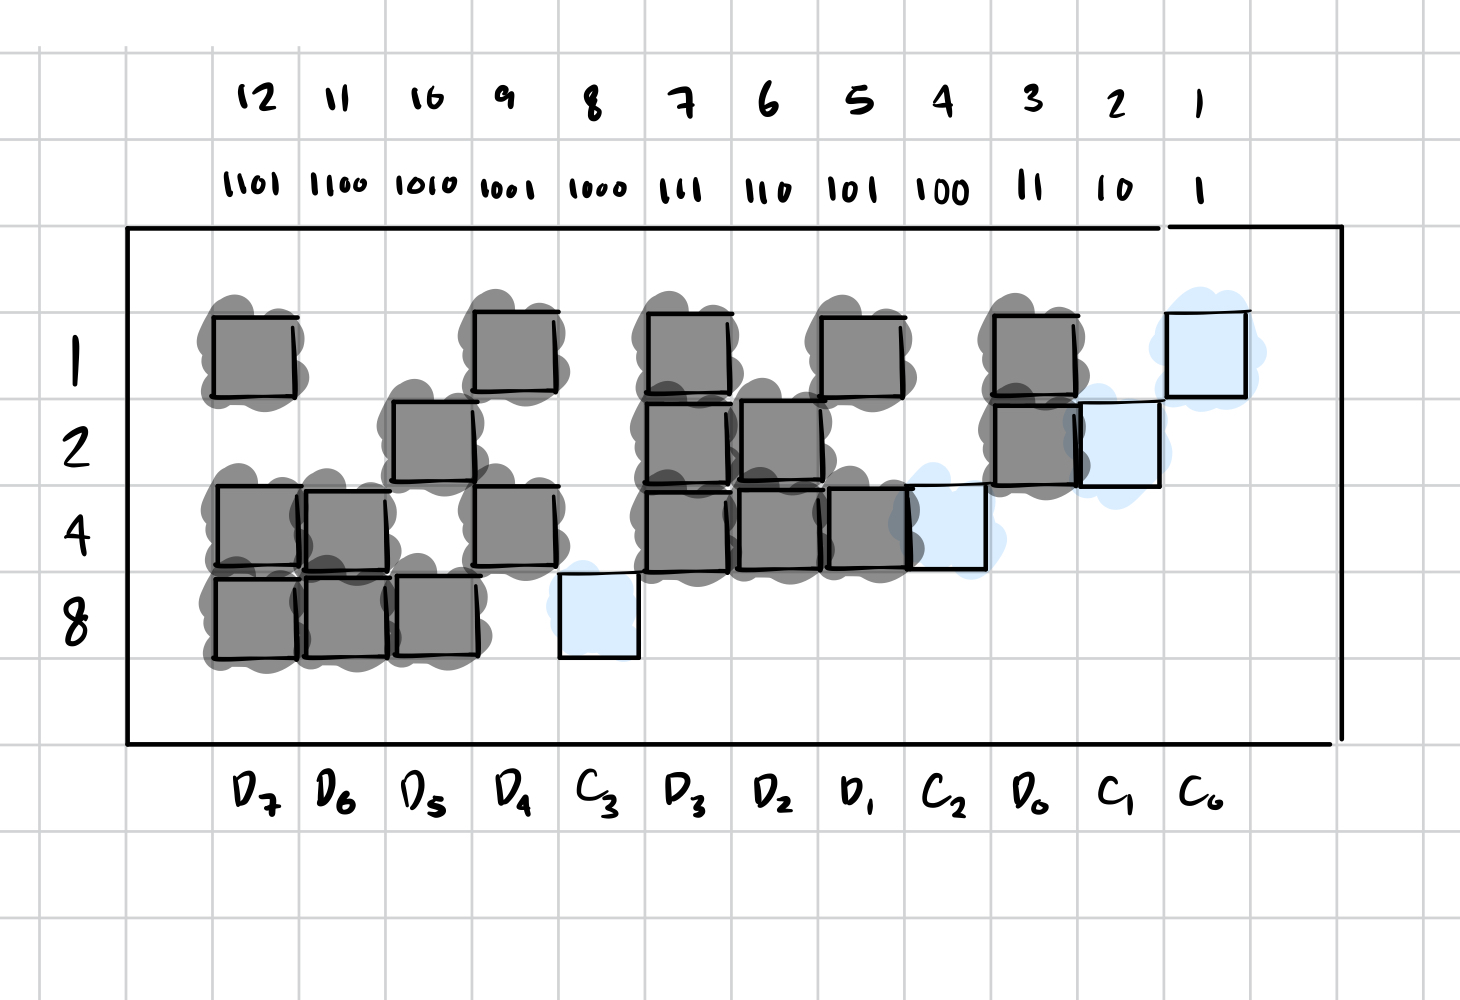
\includegraphics[width=0.8\textwidth]{homework-8_fig-2.jpg}
		  \caption{Parity-check matrix}
		  \label{fig:label}
		\end{figure}
		and the equations for calculating each check bit are
		\begin{align*}
			&C_0 = D_7 \oplus D_4 \oplus D_3 \oplus D_1 \oplus D_0 \\
			&C_1 = D_5 \oplus D_3 \oplus D_2 \oplus D_0 \\
			&C_2 = D_7 \oplus D_6 \oplus D_3 \oplus D_2 \oplus D_1 \\
			&C_3 = D_7 \oplus D_6 \oplus D_5 \oplus D_1 \oplus D_0.
		\end{align*}
		\setcounter{subsection}{16}
	\item Using the given textbook formula, we may express the Gray code values for binary numbers 0 to 15 as
		\begin{align*}
			&0_{10} \Leftrightarrow 0000_2 \Leftrightarrow 0000_{\mathrm{gray}}\\
			&1_{10} \Leftrightarrow 0001_2 \Leftrightarrow 0001_{\mathrm{gray}}\\
			&2_{10} \Leftrightarrow 0010_2 \Leftrightarrow 0011_{\mathrm{gray}}\\
			&3_{10} \Leftrightarrow 0011_2 \Leftrightarrow 0010_{\mathrm{gray}}\\
			&4_{10} \Leftrightarrow 0100_2 \Leftrightarrow 0110_{\mathrm{gray}}\\
			&5_{10} \Leftrightarrow 0101_2 \Leftrightarrow 0111_{\mathrm{gray}}\\
			&6_{10} \Leftrightarrow 0110_2 \Leftrightarrow 0101_{\mathrm{gray}}\\
			&7_{10} \Leftrightarrow 0111_2 \Leftrightarrow 0100_{\mathrm{gray}}\\
			&8_{10} \Leftrightarrow 1000_2 \Leftrightarrow 1100_{\mathrm{gray}}\\
			&9_{10} \Leftrightarrow 1001_2 \Leftrightarrow 1101_{\mathrm{gray}}\\
			&10_{10} \Leftrightarrow 1010_2 \Leftrightarrow 1111_{\mathrm{gray}}\\
			&11_{10} \Leftrightarrow 1011_2 \Leftrightarrow 1110_{\mathrm{gray}}\\
			&12_{10} \Leftrightarrow 1100_2 \Leftrightarrow 1010_{\mathrm{gray}}\\
			&13_{10} \Leftrightarrow 1101_2 \Leftrightarrow 1011_{\mathrm{gray}}\\
			&14_{10} \Leftrightarrow 1110_2 \Leftrightarrow 1001_{\mathrm{gray}}\\
			&15_{10} \Leftrightarrow 1111_2 \Leftrightarrow 1000_{\mathrm{gray}}\\
		\end{align*}
		\setcounter{subsection}{17}
	\item An N-bit gray code counter could be implemented by simply connecting the output of a binary counter to \(N\) XOR gates, as follows:
		\begin{figure}[H]
		  \centering
		  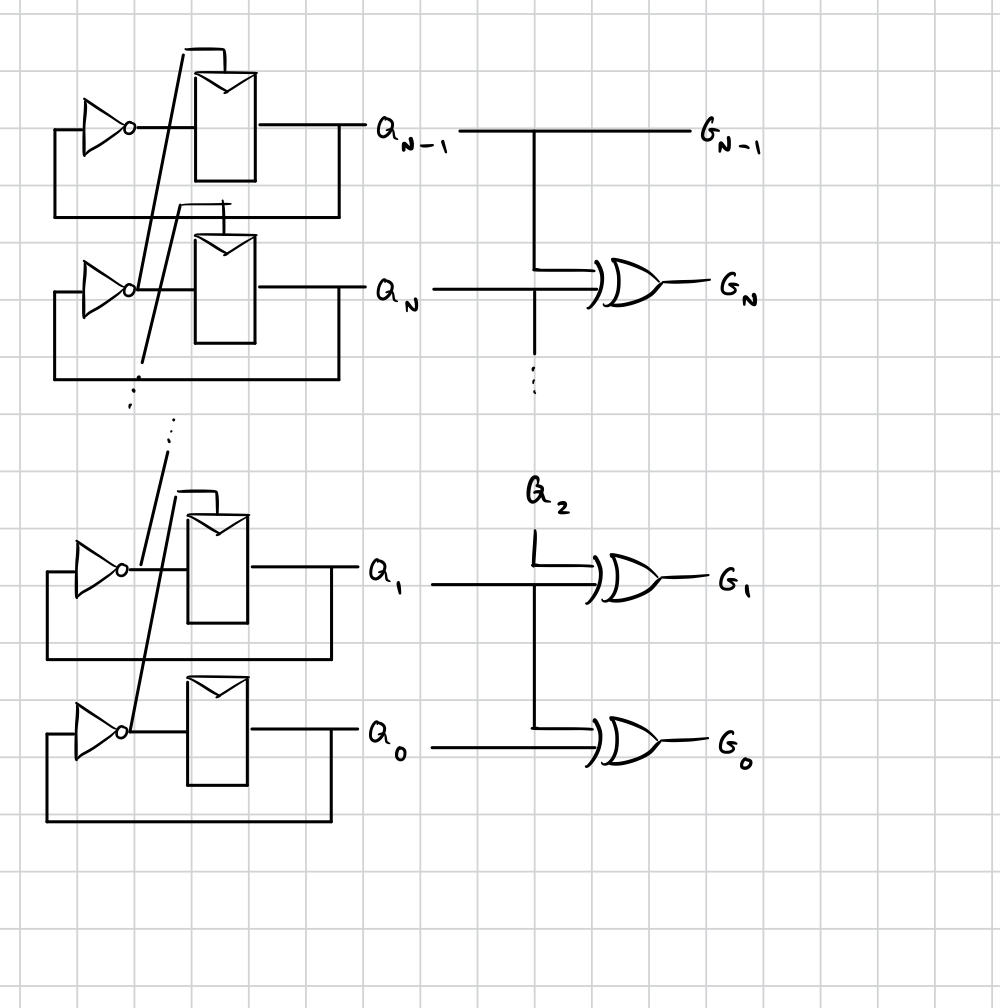
\includegraphics[width=0.8\textwidth]{homework-8_fig-1.jpg}
		  \caption{N-bit Gray code counter}
		  \label{fig:no}
		\end{figure}
		Of course, this design could be improved upon by including a reset function and reducing delay using other counter architectures, but the general idea would be the same.
\end{enumerate}
\end{document}
